%%%%%%%%%%%%%%%%%%%%%%%%%%%%%%%%%%%%%%%%%%%%%%%%%%%%%%%%%
%                                                       %
%  情報処理学会全国大会投稿論文用テンプレートファイル   %
%                   for ips.sty ver2.1                  %
%                                                       %
%%%%%%%%%%%%%%%%%%%%%%%%%%%%%%%%%%%%%%%%%%%%%%%%%%%%%%%%%

%%% ver2.1 +
%%% edited by Jutori
%%% modified by Kenta

\documentclass[a4paper,9pt, twocolumn]{jarticle}
%\documentclass[a4paper,9pt,twocolumn]{ipsjpapers}
\usepackage{graphicx}
\usepackage{ips}
\usepackage{mediabb}
\usepackage{here}

\renewcommand{\baselinestretch}{0.87}   % 行間

\pagestyle{empty}
%%%%%%    TEXT START    %%%%%%
\begin{document}

%%%%%%%%%%%%%%%%%%%%%%%%%%% ヘッダ %%%%%%%%%%%%%%%%%%%%%%%%%%
\twocolumn[%
\begin{center}

%--------------------------------------------------------------
% 講演タイトル(2行にわたるときは\2jtitle{}{}{})
%--------------------------------------------------------------

\vspace{-3mm}
\2jtitle{}{独自ベクトル処理機能を備えたプロセッサ向け}{自動ベクトル化コンパイラの開発}

%--------------------------------------------------------------
% 日本語著者名
%--------------------------------------------------------------
% name{1}{***} : 所属1の氏名
% name{2}{***} : 所属2の氏名 のようにする.所属の引数は4まで
% 名前は絶対間違えないように

\begin{authors}
\name{1}{永池 晃太朗}
\name{1}{大津 金光}
\name{1}{横田 隆史}
\name{1}{小島 駿}
\end{authors}
%--------------------------------------------------------------
% 所属
%--------------------------------------------------------------
% aff{1}{***} : 所属1
% aff{2}{***} : 所属2 のようにする.所属の引数は4まで.

\begin{affiliation}
\aff{1}{宇都宮大学工学部情報工学科}
\end{affiliation}

%--------------------------------------------------------------
\end{center}
]%

%%%%%%%%%%%%%%%%%%%%%%%%    脚注   %%%%%%%%%%%%%%%%%%%%%%%%%%

%--------------------------------------------------------------
% 英文タイトル
%--------------------------------------------------------------

\etitle{Development of automatic vectorization compiler for processors with original vector processing function.}


%--------------------------------------------------------------
% 英語語著者名
%--------------------------------------------------------------
% ename{1}{***} : 所属1の氏名
% ename{2}{***} : 所属2の氏名 のようにする.

%\ename{1}{First Last, First Last and First Last}
%ename{2}を使う場合、所属1の人と2の人で改行されてしまうので、\enameをコメントアウトして以下のように直接書くのをおすすめ (空白は適宜調節のこと)
\footnotetext{%
    \hspace{-3mm}\raise1ex\hbox{{\scriptsize \dag}}Kotaro Nagaike,%
    \hspace{1.5mm}\raise1ex\hbox{{\scriptsize \dag}}Kanemitsu Ootsu,%
    \hspace{1.5mm}\raise1ex\hbox{{\scriptsize \dag}}Takashi Yokota,%
    \hspace{1.5mm}\raise1ex\hbox{{\scriptsize \dag}}Shun Kojima,%
}
%ただし所属が3の場合は†††でなく‡となるので,\ddagと付けること
%\footnotetext{%
%    \hspace{-3mm}\raise1ex\hbox{{\scriptsize \dag}}First Last,%
%    \hspace{1.5mm}\raise1ex\hbox{{\scriptsize \dag}}First Last,%
%    \hspace{1.5mm}\raise1ex\hbox{{\scriptsize \dag\dag}}First Last,%
%    \hspace{1.5mm}\raise1ex\hbox{{\scriptsize \ddag}}First Last,%
%}
%\footnotetext{%
%    \hspace{-1mm}\raise1ex\hbox{{\scriptsize \dag\dag}}First Last and%
%    \hspace{1mm}\raise1ex\hbox{{\scriptsize \dag\dag}}First Last%
%}


%--------------------------------------------------------------
% 英語所属
%--------------------------------------------------------------
% eaff{1}{***} : 所属1
% eaff{2}{***} : 所属2 のようにする.所属の引数は4まで.
% ※日本語の所属と対応させること.
\eaff{1}{Department of Information Science, Faculty of Engineering, Utsunomiya University}


%--------------------------------------------------------------
% 英語住所
%--------------------------------------------------------------



% 上マージン30mm 下25mm 横20mm 段組の間隔 7mm
% 印刷した後、自分で確認すること

%%%%%%%%%%%%%%%%%%%%%%%% ここから本文 %%%%%%%%%%%%%%%%%%%%%%%%%%
\section{はじめに}
%%intro.tex
FPGA(Field Programmable Gate Array)はユーザによって回路の再構成が可能なLSIであり,目的の処理をハードウェアとして実装可能なデバイスである.
近年FPGAの大容量化,高性能化によって大規模な回路が実現可能になった.これによりFPGAは自動運転を始めとする組込み分野での利用増加が期待されている.

FPGAを用いたハードウェア開発はHDL(Hardware Description Language)によるRTL(Register Transfer Level)設計が広く用いられている.RTLはFPGA上に構成する回路の信号の流れや制御構造を直接設計できる一方,動作検証やデバックが難しく,短期間で複雑な処理の開発は困難である.\cite{bib:fpga}
そのため,FPGAによる開発期間を短縮する方法として,専用ハードディスクとプロセッサを用いたソフトウェアによる処理を組み合わせる方法が考えられる.FPGA上のハードウェアリソースを用いて実装するプロセッサのことをソフトコアプロセッサという.
一般的に組込みシステムではそのコストやサイズ,消費電力などに制限があるためハードウェア資源に制約があることが多く,メモリバンド幅が限られることからメモリシステムの性能が高くないことが多い.メモリシステムの性能が低いと演算性能を高くしてもメモリアクセスに時間がかかり,結果としてシステム全体の性能はメモリシステムの性能によって左右される.\cite{bib:2}
そこで,ソフトコアプロセッサによる処理を考える.すべての処理を専用ハードウェア回路で行うのではなく,高い性能の求められない汎用的な処理についてはソフトコアプロセッサにて行うことにより開発する専用ハードウェア回路を削減でき,ソフトコアプロセッサの性能が向上して専用ハードウェア回路を削減しても求められた性能に達することができればハードウェアの開発コストを抑えることができる.

組込み分野ではAI技術に注目が集まっている.独立行政法人情報処理推進機構の調査によると,将来強化/新たに獲得したい技術として組込み/IoT関連企業の46\%がAI技術を挙げている.\cite{bib:ipa}

AI技術の応用としては画像認識などの画像処理が行われる.画像処理では画像を構成する画素に対して同じ処理を行うようなものが多い.このように複数のデータに対して同じ演算を行う処理については,単一命令で複数データの処理を行うSIMD(Single Instruction, Multiple Data)や,複数命令を並列に実行するMIMD(Multiple Instruction, Multiple Data)による並列処理で高速化が可能である.\cite{bib:simd,mimd}
MIMDは複数の制御を並列化することができるため,異なる処理を同時に実行するアプリケーションでは有効である.しかし,プロセッサに複数の制御ユニットをもたせる必要があるためSIMDと比較するとハードウェアのコストが大きくなる.一方SIMDは単一の制御ユニットで複数の演算ユニットを並列動作させるため制御ユニットのコストは低くなる.
データ並列処理では複数のデータに対して同じ処理を実行するためSIMDによって並列処理が可能である.

SIMDによる並列処理を行う場合,SIMD命令は1命令で演算するデータ数が決まっている.そのため演算性能を上げるために同時演算数を変更すると機械語コードを作り直す必要がある.異なる同時演算数でも同一の機械語コードを利用可能とするためには,機械語コードが同時演算数に依存しないスケーラブルなベクトル拡張が必要である.スケーラブルなベクトル拡張により機械語コードを変更することなく,必要に応じて容易に同時演算数を増やし高性能化することが可能となる.

スケーラブルなベクトル拡張を実現したものとしてオープンな命令セットアーキテクチャであるRISC-V\cite{bib:risc-v}をベクトル拡張したベクトル拡張付きRISC-V\cite{bib:kimura}が提案されている.ベクトル拡張付きRISC-Vは組込み機器に広く用いられているARMのベクトル拡張であるARM SVE(Scalable Vector Extension)\cite{bib:arm_sve}の命令セットを参考に組み込み向けにRISC-Vに拡張したものである.しかし,ベクトル拡張付きRISC-Vに対応したコンパイラが存在していない.そこで解決策としてベクトル拡張付きRISC-Vのベクトル命令のアセンブリコードを得るためのコンパイラの開発を検討した.

本論文では,第2章で現在のMIQSプロセッサについて述べる.第3章でベクトル拡張付きRISC-V命令の生成のために利用したコンパイラ基盤であるLLVMについて述べる.第4章で実際に命令生成のための実装について述べる.第5章では実際のソースコードからアセンブリコードの出力を行った結果について述べる.       % 同一ディレクトリのintro.texが読み込まれる
画像認識等のデータ並列性の高い処理の高速化にはSIMD命令による処理が効果的である.しかし,SIMD命令による処理は同時演算数を変更する場合,同時に機械語コードを作り直す必要がある.そこで我々は機械語コードの変更なしに同時並列演算数を変更することができる,データ並列処理のためのスケーラブルなベクトル処理機能を備えたベクトル拡張付きRISC-Vを開発している\cite{bib:kimura}.

我々のベクトル拡張付きRISC-Vは,ARMのベクトル拡張であるARM SVE\cite{bib:arm_sve}を参考に組込み向けにRISC-V\cite{bib:risc-v}をベクトル拡張したものである.
これにより,機械語コードが同時演算数に依存しないスケーラブルなベクトル拡張を実現したが,これに対応したコンパイラがない.

この問題に対して,既存のRISC-Vコンパイラをベースとして,我々のベクトル拡張に対応した自動ベクトル化コンパイラを開発する手段を検討する.


\section{ベクトル拡張付きRISC-V}

我々のベクトル拡張付きRISC-VはRISC-V命令セットで定義されている4つのカスタム命令のためのオペコード領域のうち2つを利用しており,1つをベクトルロード・ストア命令,もう一方をベクトル演算命令とベクトル制御命令に使用している.

ベクトル演算命令は,プレディケート付き演算,プレディケートなし演算命令,即値による演算命令に分けられる.演算命令は,算術論理演算命令,乗除算命令,ベクトルレジスタの各要素の総和を求める命令やアドレス計算の際に用いるインデックスレジスタを生成する命令からなる.プレディケート付き演算命令ではプレディケートレジスタによるベクトルマスク制御を行う.

ベクトル制御命令はプレディケート演算命令とベクトル長操作命令に分けられる.プレディケート演算命令は,プレディケートレジスタ同士の論理演算を行う.これにより柔軟なベクトルマスク制御を行う.ベクトル長操作命令は,スカラレジスタに対しベクトル長を足す等の命令がある.ベクトル制御命令によってスケーラブルなベクトル処理を実現している.

レジスタの構成は,v0からv31のベクトルレジスタ,vp0からvp7のプレディケートレジスタ,vp8からvp15のベクトル長レジスタ,x0からx31の汎用レジスタとなっている.

\section{LLVMコンパイラ基盤}
コンパイラの開発にはコンパイラ基盤であるLLVM\cite{bib:llvm}を用いる.
コンパイラ基盤はコンパイラの各機能がモジュール化されており,機能の再利用が行いやすくなっている.
そのため,LLVMで提供されている各種モジュールを利用することで、独自機能部分の実装に集中することができる.
また,LLVMには自動ベクトル化機能が備わっており,入力ソースコードの繰り返し処理をベクトル化されたLLVM IRに変換する.ベクトル化されたLLVM IRでは,処理対象の全データへ演算を行うためにベクトル演算を繰り返した後に余剰分のデータを逐次処理によって演算を行う.
そのLLVM IRからパターンマッチングにより各ターゲットへのベクトル命令への変換などが行われる.
%RISC-VのV拡張用のパターンマッチングについても実装済みのものを再利用する.
ベクトル拡張付きRISC-VはRISC-Vを拡張しているため,LLVMのRISC-Vコンパイラとしての機能を再利用してコンパイラの開発を行う.

なお,使用するLLVMのバージョンは13.0.0である.

LLVMはソースコードから中間表現であるLLVM IRに変換を行うフロントエンド,LLVM IRからアセンブリコード生成を行うバックエンドからなる.本研究では独自命令生成のためにバックエンドに対して変更を加える.

\begin{figure}[t]
    \centering
    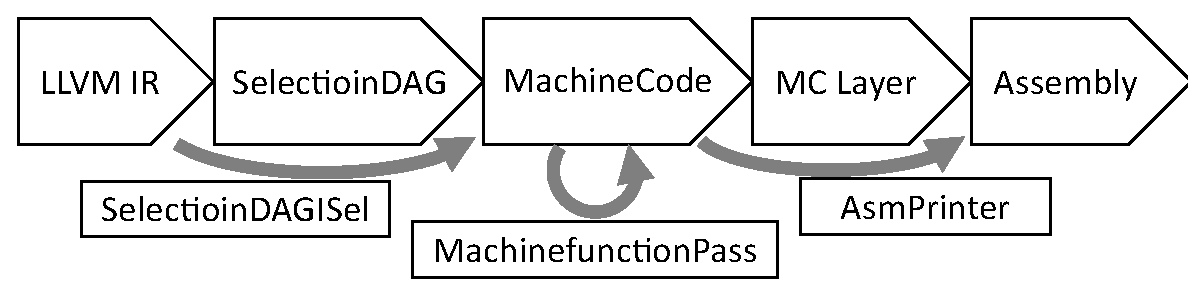
\includegraphics[scale=0.35]{backend_mojideka_2.eps}
    \vspace{-3truemm}
    \caption{コード生成の流れ}
    \vspace{-4truemm}
    \label{fig:backend}
\end{figure}

バックエンドにおけるコード生成について,処理の流れとパスを図1に示す.パスとはLLVMにおけるLLVM IR等のコードに対して最適化や変換を行うものである.
SelectionDAGフェーズではSelectionDAGISelパスによってLLVM IRをDAG(Directed Acyclic Graph)形式へと変換し,DAGのパターンマッチングによるノードの置き換えによる単純化,共通部分削除などの最適化,ターゲット命令への変換の順に行いMachineCode形式を出力する.SelectoinDAGは一つのノードが一つのLLVM IR命令に対応し,命令やデータの依存関係を表すグラフである.
MachineCode形式はターゲットが使用する実際の命令を持った形式でSSA(Static Single Assignment)形式である.SSA形式では各変数が一度のみ代入される.MachineCodeでは命令のオペランドを仮想レジスタを用いてSSA形式で表現している.MachineCodeはMachinefunctionPassによってSSAベースの最適化を行い,命令への物理レジスタの割当を行う.レジスタの割当を行った後は仮想レジスタによるSSA形式ではなく,オペランドに実際のレジスタを用いた形式となっている.

MC Layer形式はアセンブリコードに近い形式で,命令とオペランドの情報を持つ.AsmPrinterパスでアセンブリコード,オブジェクトコードを出力する際の中間表現として用いられる.

以上のLLVMバックエンドでの処理はレジスタ情報,命令フォーマットや命令のニーモニック等の情報に従って行われ,その情報はLLVMにおけるターゲットマシン情報記述のためのドメイン固有言語であるTableGenを用いて記述する.

%LLVMではRISC-VのV拡張用にTableGenによるベクトルレジスタ,ベクトル命令の定義が既に存在している.本研究ではベクトルレジスタはそのまま使用し,ベクトル命令については既存の定義に従った形式でベクトル拡張付きRISC-V命令の定義を行う.


\section{LLVMにおける独自命令の生成機能の実装}

\begin{figure}[t]
    \centering
    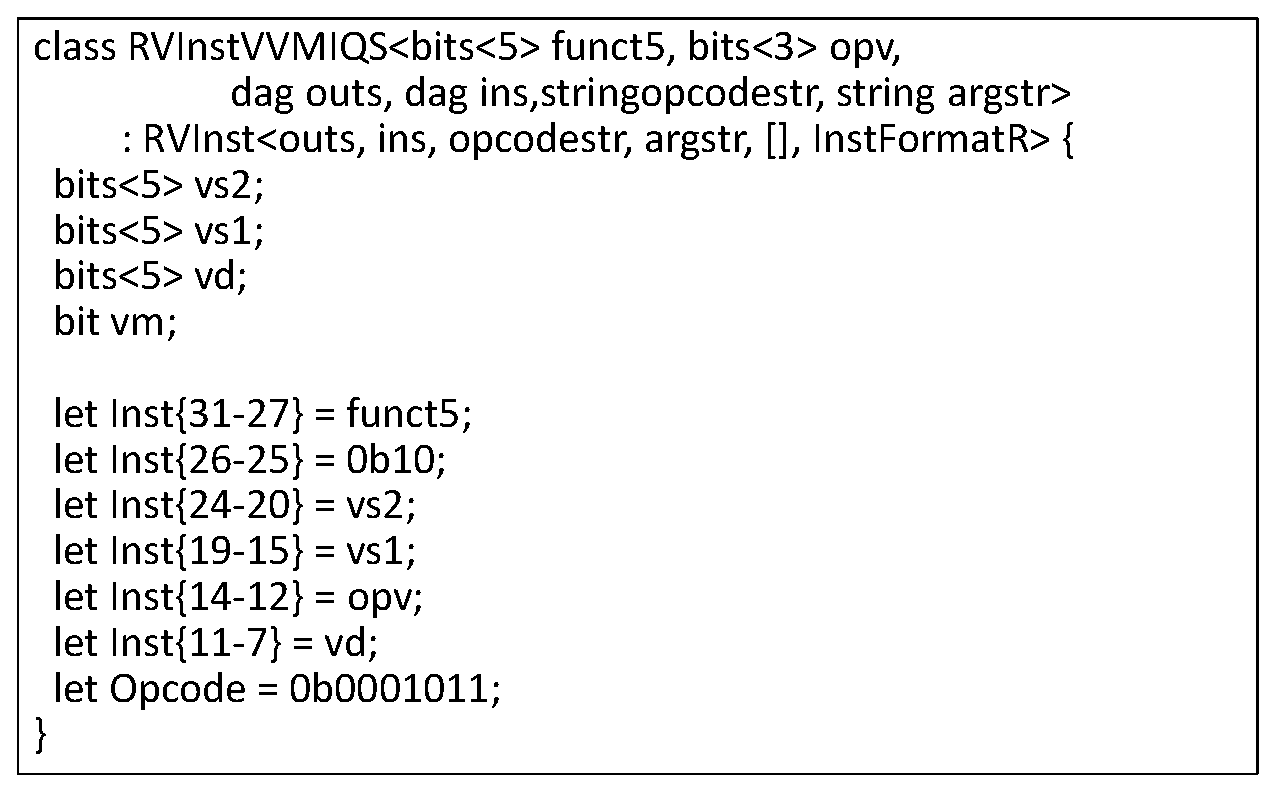
\includegraphics[scale=0.35]{RVInstVVMIQS.eps}
    \vspace{-1truemm}
    \caption{命令フォーマットの定義}
    \vspace{-2truemm}
    \label{fig:Instruciton_format}
\end{figure}

ベクトル拡張付きRISC-V命令の定義のために,図2のようなクラスを定義する.クラスRVInstVVMIQSはベクトル要素同士を演算する命令であるベクトル加算等の命令用のフォーマットとして定義する.各命令フォーマットは32bitの命令フィールドを定義している基本クラスRVInstを継承する形で命令によって異なるフォーマットを定義する.

\begin{figure}[t]
    \centering
    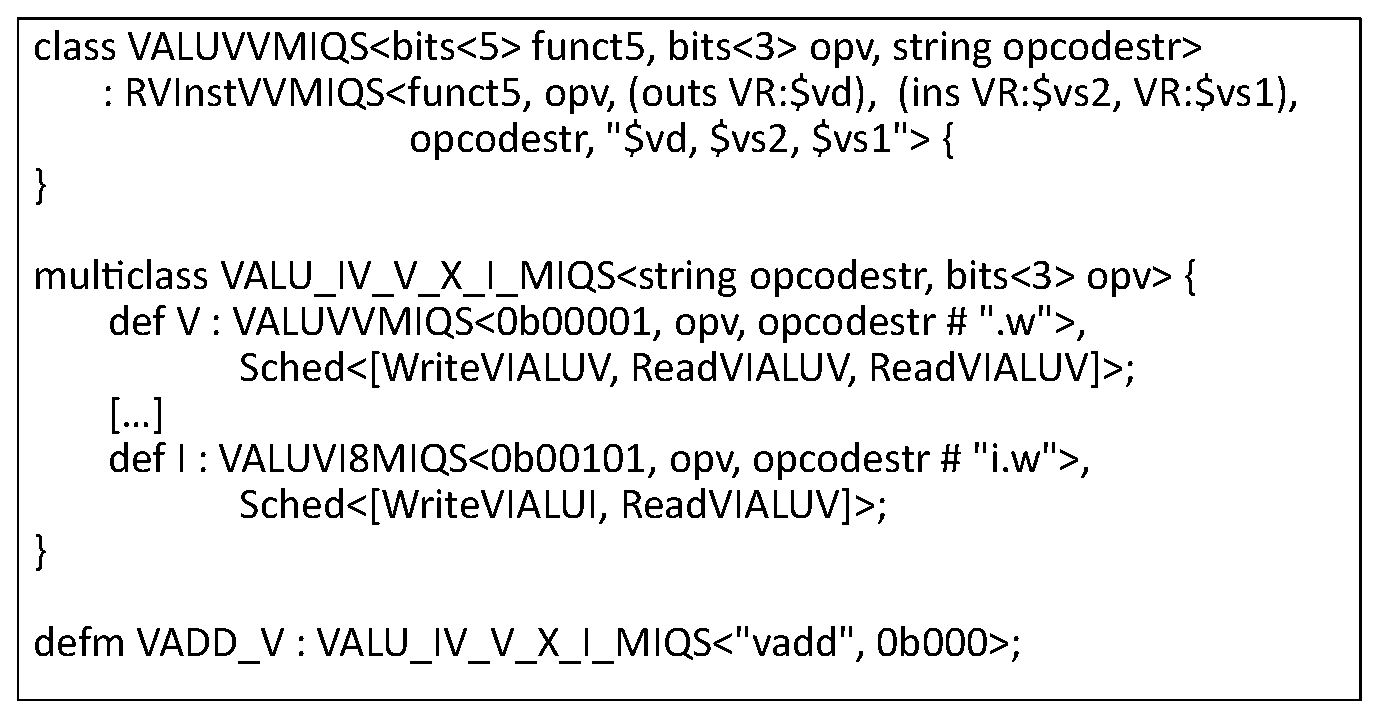
\includegraphics[scale=0.35]{Instruction.eps}
    \vspace{-7truemm}
    \caption{命令の定義}
    \vspace{-4truemm}
    \label{fig:Instruciton}
\end{figure}

命令の定義は命令フォーマットのクラスを継承し,エンコードの値やニーモニックを指定して行う.命令の定義を図3に示す.図3のVALUVVMIQSクラスは命令定義の際に同じ定義の繰り返しを防ぐために定義する.同様の入出力レジスタを持つ命令はこのクラスをインスタンス化する際に命令の文字列と命令選択に用いるための12-14ビットの値の指定を行う.

配列加算のプログラムからアセンブリコードを生成した結果の一部を図4に示す.vadd.wが我々のベクトル拡張命令のベクトル加算命令である.しかし,ロード・ストア命令についてはRISC-VのV拡張の命令のままである.

\begin{figure}[tb]
    \centering
    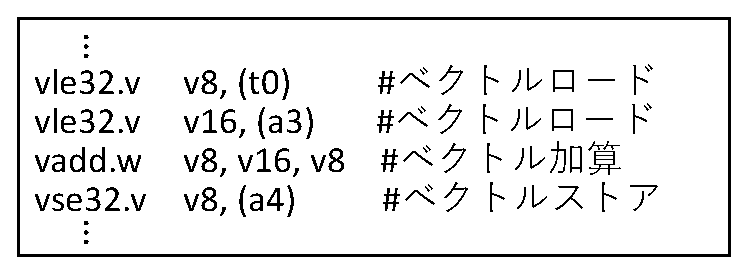
\includegraphics[scale=0.4]{miqs_assembly.eps}
    \vspace{-2truemm}
    \caption{生成されたアセンブリコード}
    \vspace{-4truemm}
    \label{fig:assembly}
\end{figure}

現在ベクトル拡張付きRISC-Vのベクトル命令の内,ベクトル演算命令のプレディケートなし,即値による演算命令の実装が完了している.しかし,ロード・ストア命令等が未実装である.それらの命令ではプレディケートレジスタを用いており,新たにプレディケートレジスタの定義を必要とする.また,現在のLLVM IRはベクトル演算の繰り返しと逐次処理によるベクトル処理を行っている.そのため,我々のベクトル拡張のプレディケート付き命令を効果的に利用できない.

\section{おわりに}
本稿では,自動でベクトル化された独自のベクトル拡張付きRISC-V命令アセンブリコードを得るためのLLVMバックエンドの実装を行った.

今後の課題として,ベクトルロード・ストア命令等の未実装の命令生成の実現が挙げられる.
現在実装済みの命令は命令の定義等で実装が可能であった.しかし,未実装の命令については現在のベクトル化されたLLVM IRからの生成が困難であると考えられる.そのため,レジスタの定義に加え,LLVM IRの生成を行うフロントエンドの変更が必要である.

\renewcommand{\baselinestretch}{0.83}\selectfont
\subsection*{\small 謝辞}
\vspace{-0.5mm}
{\small 本研究は一部 JSPS 科研費 20K11726 の援助による.}
% 科研費IDや重点はその年によって記述が変わるのでよく確認すること
% 2015年時
% 調べ方:「 科研費 教授名」でぐぐる-> 研究課題番号


%
% ------ 参考文献 ------
%
\begin{thebibliography}{9}
\itemsep -1.7pt

\bibitem{bib:kimura}
{\small Yoshiki Kimura, et al.:      % 丁寧
%{\small 氏名ほか:             % スペースが足りない場合
\newblock ``Proposal of Scalable Vector Instruction Set for Embedded RISC-V Processor,''
\newblock Proc. 2019 Seventh International Symposium on Computing and Networking Workshops (CANDARW),
\newblock Vol.1,
\newblock pp.435-439,
\newblock 2019.}

\bibitem{bib:arm_sve}
{\small Nigel Stephens, et al.:      % 丁寧
%{\small 氏名ほか:             % スペースが足りない場合
\newblock ``The ARM Scalable Vector Extension,''
\newblock IEEE Micro,
\newblock Vol.37,
\newblock No.2,
\newblock pp.26-39,
\newblock 2017.}

\bibitem{bib:risc-v}
{\small Andrew Waterman, Krste Asanovi:      % 丁寧
%{\small 氏名ほか:             % スペースが足りない場合
\newblock ``The RISC-V Instruction Set Manual Volume I: Unprivileged ISA, Document Version 2.2,''
\newblock 2017.}

\bibitem{bib:llvm}
{\small Chris Lattner, Vikram Adve:      % 丁寧
%{\small 氏名ほか:             % スペースが足りない場合
\newblock ``LLVM: A Compilation Frame-work for Lifelong Program Analysis Transformation,''
\newblock Proc. 2004 International Symposium on Code Generation and Optimization (CGO’04),
\newblock pp.75-86,
\newblock 2004.}

\end{thebibliography}

\end{document}

